\documentclass{article} % For LaTeX2e
\usepackage{nips13submit_e,times}
\usepackage{hyperref}
\usepackage{url}
\usepackage{graphicx}
\usepackage{subcaption}
%\documentstyle[nips13submit_09,times,art10]{article} % For LaTeX 2.09


\title{Unsupervised Feature Learning for Object Classification}


\author{
Laxman Dhulipala, Harry Gifford, Wangzi He \\
Department of Computer Science\\
Carnegie Mellon University University\\
Pittsburgh, PA 15213 \\
\texttt{\{ldhulipa, hgifford, wangzih\}@andrew.cmu.edu} \\
}

% The \author macro works with any number of authors. There are two commands
% used to separate the names and addresses of multiple authors: \And and \AND.
%
% Using \And between authors leaves it to \LaTeX{} to determine where to break
% the lines. Using \AND forces a linebreak at that point. So, if \LaTeX{}
% puts 3 of 4 authors names on the first line, and the last on the second
% line, try using \AND instead of \And before the third author name.

\newcommand{\fix}{\marginpar{FIX}}
\newcommand{\new}{\marginpar{NEW}}

\nipsfinalcopy % Uncomment for camera-ready version

\begin{document}


\maketitle

\begin{abstract}
A major theme in modern object recognition research has been the use of
features to boost classification techniques. Stemming from the seminal work
of Viola and Jones, features and feature learning techniques have been used
year after year to improve existing object recognition algorithms, and increase
classification rates. In this work, we implement and evaluate an object classification framework
that first learns a dictionary of features, and subsequently uses this feature basis
to represent and classify images into categories. We evaluate our classification framework
by analyzing its performance on the CIFAR-10 dataset, and also consider several optimizations
and heuristics to help boost performance.
\end{abstract}

\section{Introduction}

Object Recognition as a field has its roots firmly embedded in a long history
of research in Neuroscience. Stemming from Hubel and Wiesel's discovery in the
late 1950's of complex and simple cells, researchers have been captivated by using
techniques and ideas from neuroscience as building blocks for robust object
classification in a machine\cite{hubel}. To this end, ideas from neuroscience such as the Perceptron
algorithm, convolution neural networks and most recently, deep belief networks have all
had tremendous success in object recognition and machine learning.

A fundamental step for many object recognition algorithms is to learn hierarchies
of features from images. Learnt features from a dataset afford the algorithm designer
to then represent images in the dataset as linear combinations of the learnt features.
In some sense, this is the most natural reason to learn features, as they allow one
to transform the space of images into the space of images as represented by their features.
This transformed space typically produces better results when running object classification
algorithms - even naive classification techniques such as $k$-nearest neighbors.

Feature heirarchies can be learnt in a variety of ways, from semi-supervised learning
algorithms to fully unsupervised learning algorithms.
Our approach to feature learning relies on an elegant and simple algorithm that was
recently published by Adam Coates and Andrew Ng \cite{coates}. They propose the use
of $k$-means clustering for feature learning as it is a simple and easily paralellizable
algorithm that can be deployed at scale. In an earlier work, they show how $k$-means in
practice is highly competitive against the state-of-the-art feature learning algorithms,
often beating them \cite{coates11}. In particular, they show a surprising result that
$k$-means based feature learning with a single layer neural network achieves state-of-the-art
error rate on the CIFAR-10 dataset.


\section{Related Work}

Object classification has had a long history of research and experimental results. In
particular, many researchers in the past decade have made attempts at understanding the
CIFAR-10 dataset with varying degrees of success. In this section we first describe
several other methods for performing feature learning, consider several algorithms which
use features to boost object classification performance, and finally describe the success
of some of these methods on the CIFAR-10 dataset.

Feature learning can be split into three categories - supervised approaches
semi-supervised approaches, and lastly unsupervised feature learning.
In terms of semi-supervised approaches, perhaps the most classic approach is that of
Nigam et al. who describes how to
learn text classifiers when there are limited number of labeled examples \cite{nigam}.
They in a sense
overcome the dearth of labeled examples by using unlabeled documents to support the data.
This is a somewhat counterintuitive result, but can be rationalized by understanding that
unlabeled data, based on inferences about which class an unlabeled example belongs to can
be used to boost the joint probability distribution of features in the document. The authors
ultimately used EM (Expectation Maximization) with the assumption that the underlying data
arises from a mixture model to classify text.

Another recent feature learning approach is pioneered by Raina et al. and runs under the
moniker of Self-Taught Learning \cite{raina}. Self-Taught Learning works similarly to
the EM-based
approach described above, but makes no assumptions about the underlying distribution or
classes of the unsupervised data (there is no assumption that the unlabeled data even
contains objects that are provided in the training and test datasets). Instead, they exploit
the fact that the unsupervised data is a collection of natural images. This makes their
algorithm significantly easier to apply in practice, as one can simply take a set of labeled
examples, and augment it with an enormous unlabeled data-set of support examples.

Both approaches are interesting due to their real world practicality - which we are deeply
concerned with. Both approaches augment their small set of labeled examples with a large
number of unlabeled examples, and use the unlabeled examples to improve performance on the
test dataset. In the world, labeled examples are prohibitively costly -
therefore it is imperative to have techniques that will be almost fully unsupervised.

\section{Datasets}
We choose to evaluate our object classification algorithm on two particular datasets, CIFAR-10 and STL-10. CIFAR-10 is a standard dataset of 32x32 color images of a single object in one of ten categories. It contains 60,000 labeled images, with 50,000 for training and 10,000 for testing. \\
\\
STL-10 is a more recent dataset of 92x92 color images, again of single objects in one of ten cate- gories. However, STL-10 is better designed for unsupervised feature learning. In particular, there are three sections of the dataset: \\

\begin{itemize}
  \item 100,000unlabeledcolornaturalimages,ofwhichonlyasubsetareoneofthetencategories.
  \item 5000 training images, 500 per class.
  \item 8000 test images, 800 per class.
\end{itemize}

Notice that there are far fewer labeled images than in CIFAR-10. This makes it a better metric to compared unsupervised methods, since the feature learning stage becomes far more important than the specific supervised classfier we use at the end.

\section{Algorithm}
We now describe the image classification algorithm, based on [1]. Assume that we have a dataset with large amounts of unlabeled data from a similar domain to the classification algorithm. Notice that this assumption differs from that in semi-supervised learning in that we are not garanteed that the unlabeled data contains only examples from what we want to classify. For example, if we are classifying birds vs. planes we may have images of buildings or plants in the unlabeled data.

\begin{enumerate}
  \item Extract random patches from the unsupervised data. Normalize the patches, so that each patch has mean 0 and 		standard deviation 1. Whiten the input patches to make the covariance matrix of the each patch approximately the identity matrix. This can be done via PCA or ZCA, as described in \cite{kriz}. 
  
	\label{headings}

\begin{figure}
  \centering
  \begin{subfigure}[h]{0.45\columnwidth}
    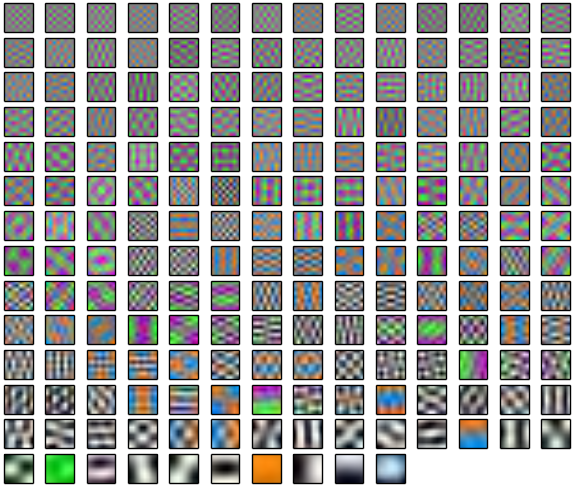
\includegraphics[width=\columnwidth]{./images/eigs192.png}
    \caption{All 192 eigenvectors of a selection of 8x8 color patches from the CIFAR dataset.}
    \label{figEigenvectors}
  \end{subfigure}
  \hspace{0.04\columnwidth}
  \centering
  \begin{subfigure}[h]{0.45\columnwidth}
    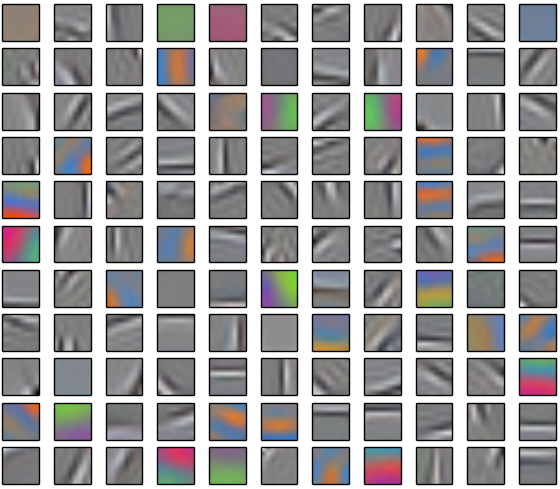
\includegraphics[width=\columnwidth]{./images/patches100.png}
    \caption{100 centroids learned from applying K-means to 8x8 patches extracted from natural images. Notice the similarity to Gabor wavelets.}
    \label{fig_centroids}
  \end{subfigure}
\end{figure}
  
  This means that we do not waste learning resources learning unneccessary imformation, such as knowing that neighboring pixels are more likely to have similar colors.
In Figure 1a we show the eigenvectors we extract when performing PCA/ZCA. We see that each eigenvector corresponds to a different frequency basis. These eigenvectors are very similar to those from the discrete cosine transform (DCT), which is often used in image compression. \\
\\
We can also optionally use PCA to reduce the dimensionality of the data. This doesn’t help with accuracy of the quality of features learned, but it does speed up the pipeline significantly.

  \item Cluster these patches using K-means with the euclidean or cosine distance metric. Gener- ally it is best to pick as large a k as the amount of data will allow, however metrics such as silhouette scoring etc. can also be useful if data is severely limited. Figure 1b shows the centroids learned when performing euclidean K-means with 100 centroids. These features are similar to those learned by blind source seperation, such as ICA \cite{hoyer}
  
  \item For each training example, extract all patches from each image. Normalize and whiten these patches as in 1. Get some measure of ‘distance’ from the centroids learned by K- means. There are many approaches that can be taken here. For example, we can find the euclidean distance to each patch or convolve each centroid with the whitened patches from the image. We can also use the distance metric suggested by Coates which has the benefit of adding some sparsity: $f_{ij} = $max(0, $\mu_i - x_{ij}$), where $\mu_i$ is the average distance from the patch to each centroid and $x_{ij}$ is the distance from patch i to centroid j.
  
  \item Pool these feature responses in order to reduce the dimensionality. One approach is to pool the responses into a n $\times$ n grid.
  
  \item Pass these features into your favorite linear classifier (e.g. SVM or logistic regression) or pass these features back into the K-means pipeline described above.
\end{enumerate}

\newpage

\bibliographystyle{acm}
\bibliography{ref}



\end{document}
